\documentclass{standalone}

\usepackage{xcolor}
\usepackage{bm}
\newcommand{\mat}[1]{\bm{#1}}

\usepackage{tikz}
\usepackage{tikz-3dplot}

\begin{document}

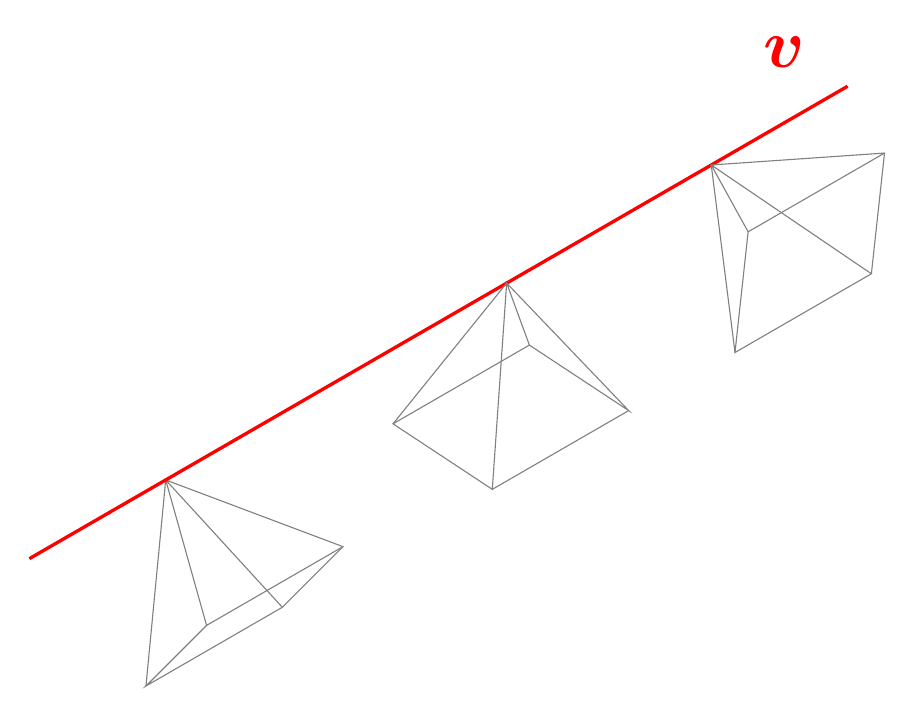
\begin{tikzpicture}
\begin{scope}[rotate around z=30]
\begin{scope}[rotate around x=00, shift={(0,0,0)}]
\draw[color=gray] (0,0,0) -- (-1,-2,-1) -- (-1,-2,1) -- (1,-2,1) -- (0,0,0) -- (1,-2,-1) -- (1, -2, 1);
\draw[color=gray] (0,0,0) -- (-1,-2,1);
\draw[color=gray] (-1,-2,-1) -- (1,-2,-1);
\draw[very thick, color=red] (-2,0,0)--(10,0,0) node[above, xshift=-8mm, yshift=1mm]{\Huge\color{red}$\mat{v}$};
\end{scope}

\begin{scope}[rotate around x=-50, shift={(5,0,0)}]
\draw[color=gray] (0,0,0) -- (-1,-2,-1) -- (-1,-2,1) -- (1,-2,1) -- (0,0,0) -- (1,-2,-1) -- (1, -2, 1);
\draw[color=gray] (0,0,0) -- (-1,-2,1);
\draw[color=gray] (-1,-2,-1) -- (1,-2,-1);
\end{scope}

\begin{scope}[rotate around x=30, shift={(8,0,0)}]
\draw[color=gray] (0,0,0) -- (-1,-2,-1) -- (-1,-2,1) -- (1,-2,1) -- (0,0,0) -- (1,-2,-1) -- (1, -2, 1);
\draw[color=gray] (0,0,0) -- (-1,-2,1);
\draw[color=gray] (-1,-2,-1) -- (1,-2,-1);
\end{scope}
\end{scope}

\end{tikzpicture}
\end{document}
